\chapter{智能网联安全与威胁建模}
\label{ch3}

\section{智能网联汽车面临的安全威胁}
安全性是智能网联汽车面临的迅速出现的重大挑战。在车载网络的背景下,安全问题通常是指通信数据可能被恶意攻击者窃听、欺骗、丢弃、修改、泛滥、窃取等危险情况。
在车辆向自动驾驶和协作驾驶发展的时代,安全性在车载网络的设计中变得越来越重要。
\subsection{智能网联汽车主要攻击手段}
发明车载网络协议时,安全问题并不是主要问题。因此,许多安全功能天生就缺失了。例如,CAN 缺乏必要的保护来确保信号的可用性、机密性和真实性\cite{woo2014practical}。
FlexRay 虽然能够在出现错误的情况下保持正确操作,但无法抵御格式良好的恶意错误消息\cite{kleberger2011security}。尽管如此,这些缺点在过去并未构成迫在眉睫的安全威胁,因为车辆很少与外界连接,
而老式的安全攻击通常需要对车载网络进行物理访问。

然而,现代车辆正在通过各种方式迅速变得更加互联,用于许多高级应用。例如,车辆可以通过 DSRC(专用短程通信)连接以实现 VANET(车载自组织网络)功能,
通过 Wi-Fi/蓝牙实现车载娱乐,并通过蜂窝网络实现远程信息处理服务。尽管这些连接使车辆更加智能和舒适,但它们也将车载网络大量暴露给外部对手。
例如,CAN 通信可能会被智能手机恶意软件通过蜂窝网络远程篡改\cite{woo2014practical}。软件病毒可能通过受感染的娱乐媒体(如 CD(光盘)或蓝牙播放器)传播到车载组件。
此外,还可以通过攻击OEM存储中心的ECU密钥管理不善来侵入车载网络。

此外,直接访问的威胁仍然存在,因为攻击者也可能物理侵入通信线路,直接针对网络组件的弱点发起攻击。这种典型的攻击可能包括反汇编可执行代码和将恶意代码注入运行时环境。

车载网络的安全漏洞不仅可能对车辆用户造成严重后果,还会对其他道路交通参与者造成严重后果。例如,安全漏洞可能导致车辆用户的隐私泄露。目标私人数据可能包括车辆诊断流
、机柜对话、摄像记录、驾驶模式和车辆位置\cite{amoozadeh2015security}. 
这种典型的攻击是通过未经授权的窃听进行的。其次,安全漏洞可能导致车主或原始设备制造商的直接金钱损失。在此类攻击中,
攻击者经常故意修改或重放所需的车载数据以实现非法收益,例如车辆盗窃或里程表欺诈。第三级安全漏洞可能会对车辆使用者造成安全威胁。
这种攻击通常涉及对安全关键车载数据的恶意修改或伪造,例如轮胎压力、车速、发动机扭矩请求和制动命令. 
这可能导致非自愿驾驶机动甚至交通事故。考虑到自动驾驶的出现,这种危险至关重要,值得研究界更多关注。
第四,车载网络安全漏洞会对其他道路参与者造成安全威胁,甚至瘫痪整个交通系统。由于车辆将在大型网络中互连,
例如 VANET,因此信号可信度对于协调交通系统中的所有车辆都极为重要\cite{harding2014vehicle}.
 但是,如果车载网络安全受到损害,这种可信度可能会被破坏。
 例如,被篡改的车载网络可能会产生虚假数据,如果虚假数据已经传播到车辆外部并被其他人认为是“值得信赖的”,则可能对其他车辆造成极大的危险。
综合上述研究现状,将攻击手段分为以下类型:
\begin{itemize}
    \item 远距离通信攻击: 如利用蜂窝网络、Wi-Fi等进行伪装拦截通信信号等从而达到攻击的目的。
    \item 近距离车外通信: 利用蓝牙攻击和高频无线电攻击。如通过蓝牙连接车载娱乐系统,伪装发送信号给车载娱乐系统从而达到攻击的目的。
    \item 车辆内部网络: 如通过车辆内部USB攻击IVI系统等。
\end{itemize}

\subsection{ICV 中的潜在威胁}
在远距离通信中,恶意攻击者入侵汽车的方
式大致可分为 4 种:蜂窝网络、Wi-Fi、车载单元
(OBU,on board unit)/路侧单元(RSU,road side
unit)和全球定位系统(GPS,global positioning
system)。
\newline
1) 蜂窝网络
蜂窝网络解决了 ICV 远程通信的难题,也造成
了一些安全隐患。如通过破解了汽车固件,
实现了对汽车设备(方向盘等)的远程控制。
通过无线通信信道实现了对车辆的远程控制、位置
跟踪和通信监控。
\newline
2) Wi-Fi
入侵者利用 Wi-Fi 连接可以进行很多恶意操
作。如利用 Wi-Fi 远程访问车内网络;在信息娱乐
控制台植入恶意软件;对汽车 Wi-Fi 的网络流量进
行监控。在文献\cite{keen}中,腾讯科恩安全实
验室研究员远程入侵了特斯拉汽车的网关、BCM 和
自动驾驶系统。并可以实现远程开启特斯拉电动车的天窗、车门以及在行驶中启动刹车。
通过安全漏洞,无物理接触远程成功攻入特斯拉车电网络,
并实现对特斯拉进行任意的车身和行车控制。
\newline
3) OBU/RSU
OBU 和 RSU 是利用专用短程通信技术建立微
波通信链路来实现车辆识别和电子支付功能的设
备。然而,它们在为用户出行带来方便的同时,也
产生了一些安全隐患,文献\cite{yongsai}揭露了针对新兴互
联车辆的交通信号控制的拥塞攻击。
\newline
4) GPS
GPS 是汽车导航中不可缺少的一部分。在无人
驾驶中,GPS 导航作为汽车的“大脑”,能够为汽
车提供最佳的行驶路线,因此,保证 GPS 的安全是
无人驾驶领域的一项重要工作。文献\cite{cuigai}展示了使用
便携式 GPS 欺骗器篡改车辆的 GPS 路线,严重威
胁 GPS 的安全。
\subsection{近距离车外通信的潜在威胁}
在近距离车外通信中,恶意攻击者入侵汽车的
方式可分为蓝牙攻击和高频无线电攻击两类。
\newline
1) 蓝牙攻击
蓝牙作为一种近距离数据交换的通信方式,也
是恶意攻击者关注的一个攻击面。攻击者能够利用
蓝牙接口在汽车的信息娱乐单元上执行恶意代码,
从而实现对车辆内部网络的渗透和攻击。文献\cite{antian}
利用蓝牙漏洞,开发出一款名为“BlueBorn”的攻
击向量,实现了对IVI系统的控制。
\newline
2) 高频无线电攻击
随着高频无线电在 RKE、无钥匙点火等电子元
件中的应用,很多攻击者开始关注利用高频无线电
实现欺骗攻击的方法。通过软件无线电
欺骗实现了对RKE系统的攻击,文献\cite{wuxiandian}则使用软
件无线电欺骗实现了对汽车 TPMS 系统的攻击。

\subsection{车辆内部网络的潜在威胁}
车辆内部网络的攻击面大致可分为 USB 接口
和 CAN 接口两部分。
\newline
1) USB 接口
在 ICV 中,USB 接口可以直接与 IVI 连接,实
现自动播放音频和视频文件的功能。因此,攻击者
可以在网约车、出租车等平台以播放音乐为借口,
悄悄向车内植入木马病毒从而实现对汽车的控制。
2015 年,黑客曾利用 USB 攻击造成马自达汽车 IVI
系统瘫痪。
\newline
2) CAN 接口
CAN 总线是 ECU 之间信息传输的通道,ECU
和 CAN 总线协同工作可以监控车辆状态和车辆行
为,然而,CAN 总线具有一定的脆弱性。目前,许
多汽车都安装有辅助设备(如保险狗、Mobileye、
ELM327 等),它们具有为用户提供车道偏离警告、
前方碰撞警告和车速预警等功能。攻击者可以利用
这些辅助设备的脆弱性,通过 Wi-Fi 发送控制指令,
这些设备能够将指令传输到 CAN 总线,从而使攻
击者实现对车辆状态的远程控制。文献\cite{koscher2010experimental}利用侧信
道攻击,通过收集 CAN 总线的数据流量窃取驾驶
员的隐私信息,验证了 ICV 中的用户隐私信息存在
被泄露的风险。


\section{威胁建模方法论}
威胁建模被定义为根据业务和技术利益相关者的输入,主动识别和解决对组织系统的潜在威胁的过程。通常在设计产品或新功能时完成,以避免将来出现安全漏洞的成本。

威胁建模是分析系统的各种业务和技术要求、识别潜在威胁并记录这些威胁对系统的脆弱程度的过程。威胁是指未经授权的一方访问组织的敏感信息、应用程序或网络的任何情况。 
威胁建模过程的目的是清楚地了解组织的各种资产、对这些资产的可能威胁,以及如何以及何时可以减轻这些威胁。威胁建模的最终产品是一个强大的安全系统。 
2020 年 4 月,视频通讯应用 Zoom 的股价从 159.56 美元跌至 111.41 美元。一旦用户群增加,Zoom 的许多安全漏洞就会暴露出来——其中大部分是 Zoom 没有预料到的。
2020 年 7 月,Twitter 以一组具有内部系统访问权限的员工为目标而遭到黑客攻击,导致 当时通过比特币汇款的用户损失了 117,000 美元。 
有了这样的安全攻击,品牌就会失去资本和信任。恶意软件攻击事件不会很快停止。
Cyber​​security Ventures 预测\cite{apache1},到 2021 年,网络犯罪损失每年将给全世界造成约 6 万亿美元的损失。这正是威胁建模过程可以在很大程度上减轻这些风险的地方。 
\newline
举例来说,在智能网联汽车中手机APP存储用户信息的过时加密算法是威胁建模的一个应用。
\begin{itemize}
    \item 漏洞是MD5等过时的加密算法。
    \item 威胁是使用暴力破解散列密码。
    \item 攻击者是试图在线出售个人信息的黑客。
    \item 缓解策略是将加密算法更改为更现代和更强大的东西。
  \end{itemize}
威胁建模可以通过三种不同的方式进行: 
\newline
以资产为中心:盘点各种资产,分析每个资产的脆弱性。
\newline 
以攻击者为中心:考虑可能的攻击者、每个人想要攻击的资产以及如何攻击。
\newline
以软件为中心:关注系统设计、数据如何在各个层之间流动以及如何配置
\subsection{威胁建模步骤}
要进行有效的威胁建模,首先需要以下利益相关者的意见:
\begin{itemize}
    \item 提供应用程序的业务影响的业务利益相关者。
    \item 架构师提供应用生态系统的概述。
    \item 用于特定代码输入的程序员,例如使用的框架、编码指南等。
    \item DevOps提供服务器和网络配置的详细信息。
    \item 专家学者在关键参数上的影响因子
  \end{itemize}
  其次是威胁建模的具体步骤,图3.1是威胁建模的步骤图:
  \begin{itemize}
    \item 设计:明确系统的所有要求,并创建数据流关系图。
    \item 中断: 将威胁建模框架应用到数据流关系图,并查找潜在的安全问题。
    \item 修复: 确定如何正确组合安全控制来解决每个问题。
    \item 验证: 验证是否满足了要求、找到了问题并实现了安全控制。
  \end{itemize}
  \begin{figure}
    \centering
    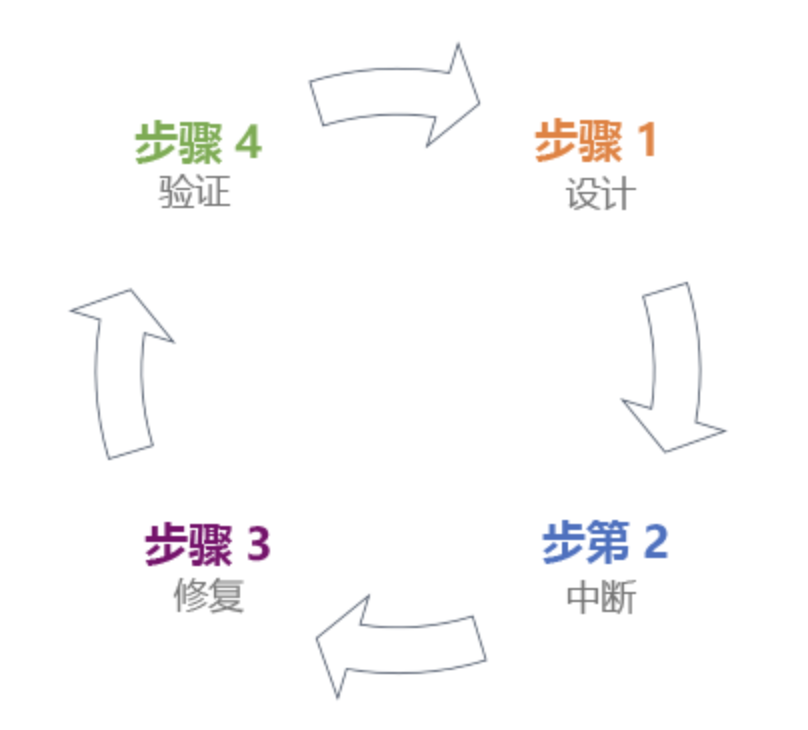
\includegraphics[scale=0.6]{resources/img/i4.png}
    \caption{威胁建模步骤}
  \end{figure}

\subsection{设计}
设计阶段是进行威胁建模活动的基础。 你需要尽可能多地收集关于你所构建的内容及所用资源的数据。
清楚地了解系统的工作原理,列出系统使用的每个服务,枚举有关环境和默认安全配置的所有假设,使用正确的上下文深度级别创建数据流关系图。
尽可能多地提出有关系统的问题。 可以考虑以下问题:
保护数据免受未经授权的披露的机密性。
防止未经授权的信息更改的完整性。
即使系统受到攻击也能提供所需的服务。
系统如何处理密钥、证书和凭据?
需要保护哪些商业秘密和知识产权?
想在威胁建模上花费多少时间和金钱?
\newline
在设计阶段"可视化"是非常重要的步骤.对整个应用程序的清晰记录的概述将大大简化流程。这包括记下用例、数据流、数据模式和部署图。您可以构建两种类型的可视化。
数据流图:它描述了数据是如何设计为在您的系统中移动的。它显示了操作级别,并清楚地显示了数据进入和退出每个组件的位置、数据存储、流程、交互和信任边界。 
流程图:它描述了用户如何在各种用例中交互和移动。它处于应用程序级别。DFD 专注于系统内部的工作方式,而 PFD 则专注于用户和第三方与系统的交互。您可以选择其中之一或同时使用两者。
这里介绍下创建数据流关系图: 数据流关系图是系统的图形表示形式,应指定每个元素及其交互和上下文。
数据流关系图显示了给定系统中的数据流。 它通常以用户或数据存储的请求开始,以数据存储或 Analytics Services 结束。 数据流关系图使用不同的形状来指示它们所表示的元素。
如元素:过程一般用圆形来表示,其定义:接收、修改输入或将输入重定向到输出的任务,如 Web 服务。
外部实体用矩形来表示,其定义:直接控制之外的任务、实体或数据存储,如用户和第三方 API。
数据存储一般用形如"二"汉字来表示,其定义:永久和临时数据存储,如 Web 缓存和 Azure 托管数据库。
数据流关系图应当包含:正在构建的系统类型和安全团队所需的上下文。	

\subsection{中断}
在中断阶段,需使用数据流关系图查找针对系统的潜在威胁。 此过程使用威胁建模框架,以帮助你查找最常见的威胁和防范威胁的方法。
选择以“保护系统”或“了解攻击者”为核心的方法, 如使用微软的STIRIDE威胁模型识别常见威胁。
选择重点领域和相关框架,以系统地识别系统中的潜在威胁。

\subsection{修复}

在修复阶段,需要决定如何处理所有威胁。 比如每个STRIDE威胁都对应到一项或多项安全控制,这些控制措施提供不同的功能和类型供你选择。
并且获得与每个资产及其操作相关的威胁的主列表或库以及可能的攻击者配置文件列表。
具体来讲:该阶段目标如下:
\begin{itemize}
    \item 根据优先级框架或安全 bug 栏衡量每个威胁的优先级
    \item 将每个威胁作为任务或工作项进行跟踪
    \item 生成对应于 STRIDE 威胁的安全控制建议
    \item 选择一项或多项安全控制类型和功能来应对每个威胁
    \item 解决任务
  \end{itemize}

\subsection{验证}

验证阶段是威胁建模过程的最后一步,通常发生在部署系统之前。 它涉及到确保满足要求、验证假设以及准备好安全控制。
确认系统满足所有新旧安全要求,配置云提供商、操作系统和组件以满足安全要求,确保使用正确的安全控制解决所有问题,在部署前对系统进行手动和自动验证。
在验证期间,需要我们检查是否所有漏洞都已得到解决。并自问以下问题:所有的威胁都被缓解了吗?是否清楚地记录了剩余风险?
完成此操作后,需要决定管理已识别威胁的后续步骤,并决定下一次威胁建模迭代的时间。
威胁建模不是一次性活动。它需要在预定的时间间隔或在应用程序开发的特定里程碑期间重复。

\section{常用威胁建模方法}

常见的威胁建模方法有:基于攻击树模型的威胁建模和 STRIDE 威胁建模。攻
击树模型是 Schneier Bruce 在上世纪末提出的一种威胁建模方法\cite{schneier1999attack},其年代久远,
理论也日益完善。此方法使用树形结构搭建攻击模型,让建模人员从面临黑客攻击
的角度考虑问题,树形结构的每一个节点,都必须被慎重考虑和布局,因为每个节
点的配置稍有不慎,都有可能被黑客攻击。攻击树模型的优点是可以利用简单的网
络模型构建复杂的威胁类型和攻击方式,其扩展性强。这样的结构,还可以从深度
优先和广度优先不同的策略来考虑问题。当整个攻击树模型足够完整时,就可以很
好的预防威胁,抵御非法攻击。不过,其劣势也非常明显,由于攻击树模型完全是
从黑客的角度来思考问题的,因而,建模者必须要具备很强的技术能力,并且有较
好的攻击经验,所以难易大规模实施基于攻击树模型的威胁建模。
1999年微软内部发表了《The threats to out products》\cite{kohnfelder1999threats}的文章,
为定义Windows全系列产品面临的安全威胁正式提出了STRIDE。
随着2002年比尔.盖茨著名的《可信任计算备忘》发布,微软承诺改善软件产品的安全性,
随即正式在SDL(安全开发生命周期)中采用了威胁建模。
\newline
通过威胁建模,我们能够实现以下这些价值:
\begin{itemize}
    \item 识别体系化的结构缺陷:大多数安全问题是设计缺陷问题,而不是安全性错误。威胁建模能帮助识别这些设计缺陷,从而减少风险敞口,指导安全测试,并降低因安全漏洞而造成的品牌损害或财务损失等可能性。
    \item 节约组织安全成本:通过对威胁进行建模,并在设计阶段建立安全性需求,降低安全设计缺陷导致的修复成本。在需求管理和威胁分析阶段,与业务开发团队高效互动,释放安全团队的专业能力,专注于高性价比的安全建设。
    \item 落地DevSecOps(开发、安全和运营)文化:通过威胁建模跑通开发和安全工具的流程集成,把风险管理嵌入产品的完整生命周期,从而推动形成完整的DevSecOps工具链。
    \item 满足合规要求:威胁建模是国际安全行业通用的方法论,通过向管理层和监管机构提供产品的风险管理活动的完整记录,帮助团队遵守全球法律法规要求,包括PCI DSS、GDPR、HIPAA、CSA STAR等。
  \end{itemize}

\subsection{STRIDE威胁模型}
\subsubsection{六类威胁}

STRIDE是从攻击者的角度,把威胁划分成6个类别,分别是Spooling(仿冒)、Tampering(篡改)、Repudiation(抵赖)、InformationDisclosure(信息泄露)、Dos(拒绝服务)和Elevation of privilege (权限提升)。

\subsubsection{四类元素}

我们在来了解下四类元素,STRIDE威胁建模的第一步就是绘制数据流图,数据流图是由【外部实体】、【处理过程】、【数据存储】、【数据流】这四类元素组成。
STRIDE威胁建模的核心就是使用这四类元素绘制数据流图,然后分析每个元素可能面临的上述六类威胁,针对这些威胁制定消减方法。

四类元素的介绍如下:

1.  外部实体

系统控制范围之外的用户、软件系统或者设备。作为一个系统或产品的输入或输出。在数据流图中用矩形表示外部实体。

2.  处理过程

表示一个任务、一个执行过程,一定有数据流入和流出。在数据流图中用圆形表示。

3.  数据存储

存储数据的内部实体,如数据库、消息队列、文件等。用中间带标签的两条平行线表示。

4.  数据流

外部实体与进程、进程与进程或者进程与数据存储之间的交互,表示数据的流转。在数据流图中用箭头表示。

使用以上四个元素绘制完数据流图后,还需要引入信任边界,安全的本质就是信任问题,信任边界往往就是攻击发起的地方。在数据流图中可以用红色的虚线隔离出信任边界。

图3.2是一个比较简单的数据流图演示:
\begin{figure}
    \centering
    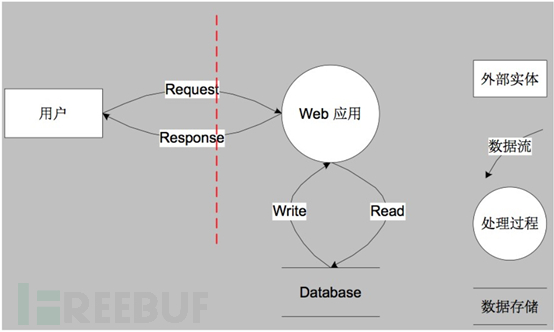
\includegraphics[scale=0.6]{resources/img/i5.png}
    \caption{简单数据流图实例}
  \end{figure}


\subsubsection{STRIDE四类元素与六类威胁的对应关系}

具体的对应关系如图3.3示例,并不是每个元素都会面临6个威胁,比如外部实体只有仿冒和抵赖两类威胁,我们不用关心外部实体会不会被篡改、会不会发生信息泄露、以及拒绝服务等,因为外部实体本来就是我们控制范围之外的。

其中进程(处理过程)会面临全部的6个威胁,数据存储中Repudiation(抵赖)是红色,表示只有存储的数据是审计类日志才会有抵赖的风险,存储其他数据的时候无抵赖。
\begin{figure}
    \centering
    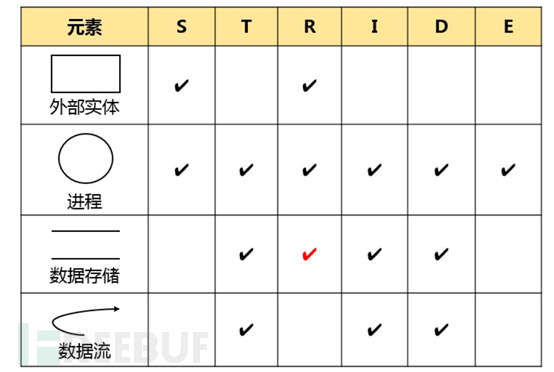
\includegraphics[scale=0.6]{resources/img/i6.png}
    \caption{四类元素和六类威胁对应关系}
  \end{figure}

\subsubsection{STRIDE 威胁建模流程}
(1) 分解业务场景,画出数据流关系图(DFD)威胁建模针对的是具体场景,
所以应该根据实际应用场景对业务进行分类,比如购买场景和注册场景等。至于有
多少个场景或怎么分类是根据用户使用的系统以及业务息息相关。比如淘宝、京东
与拼多多等电商系统,国外 Amazon EC2 和国内的腾讯云系统。这些系统分解出的业务场景肯定是不相同的。每种业务每种场景对应的
STRIDE 威胁建模是独立、互不干扰的,因此需要对分解完业务场景的每一个场景进
行单独的 STRIDE 威胁建模。接着就需要绘制数据流关系图。数据流关系图由数据
流(箭头)、数据存储(双横线)、进程(圆形)和外部实体/交互方(方形)四个元
素标准符号组成。如图 3.4 所示。
除了上述四种核心组件外,根据实际情况,可能还需要增加一个元素,称为信
任边界,在途中我们用虚线表示。当数据流在不同的信任边界上流动,就需要用虚
线来区分不同的信任区域。由于信任边界在后续的建模威胁分析种,多数不会被分
析,因此,核心元素大多只包含:进程、数据存储、数据流和交互方/外部实体四钟,
并不包含所谓的信任边界。添加信任边界后,需要对每一个节点每一段数据流进行
分析,判断是否存在 6 个维度的安全威胁。

\begin{figure}
    \centering
    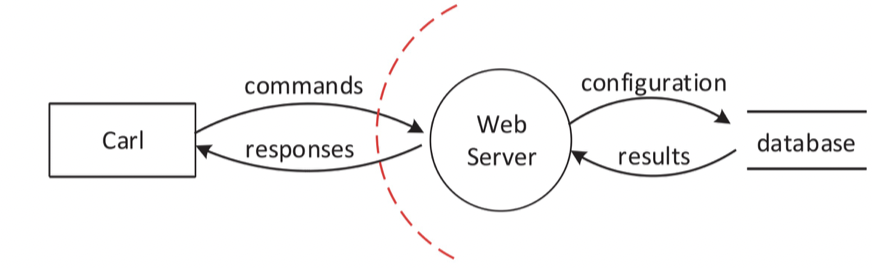
\includegraphics[scale=0.6]{resources/img/i7.png}
    \caption{常用web场景数据流图}
  \end{figure}
  (2)列出节点元素的安全威胁,逐个具体分析。绘制完数据流图之后,需要列
  出数据流中的每个节点元素可能面临的安全威胁,并逐个分析,当然也不是需要对
  每个元素的 STRIDE 威胁都要进行分析。如表 4.3 所示。
  表中列出了每种元素可能面临的安全威胁,从中能够看出只有进程才有可能面
  临 STRIDE 所有威胁,即需要对六种威胁逐个分析。外部实体可能面临“伪装”和
  “抵赖”两种威胁,数据流需要分析“篡改(替换)”、“信息丢失或泄露”和“拒绝
  服务”三种威胁。需要注意的是 R 选项勾选的是不一样的颜色,对于数据存储这个
  元素,意思是“抵赖”这个威胁可能有,也有可能没有,当数据用作审计的时候,需
  要分析“抵赖”威胁,其他情况不需要考虑这个威胁。
  \begin{center}
    \begin{tabular}{|l|l|l|l|l|l|l}
      \hline 元素类型 & 伪装 & 篡改 & 抵赖 & 信息泄露 & 拒绝服务 & 权限提升\\
      \hline 外部实体 & X & X & X & X & X & X \\
      \hline 进程 & X & X & X & X & X & X \\
      \hline 数据存储 & X & X & X & X & X & X \\
      \hline 数据流 & X & X & X & X & X & X \\
      \hline
      \end{tabular}
  \end{center}
  
  (3)输出威胁列表包括消减方案和威胁评级。分析完数据流图中所有元素即所
有对象的潜在安全威胁之后,需要输出一个威胁列表。如表4.4 就是一个典型的威胁
列表。威胁列表本身不能说是一个方法论,只能说是相关工作的结果,是威胁建模
中一个辅助的列表,能够帮助我们进一步分析威胁,进一步提高威胁建模的准确度。
其中,消减方案和危险评级是需要重点分析的两项。
\begin{center}
  \begin{tabular}{|l|l|}
    \hline 组件(威胁的目标) & App 应用程序用户身份验证进程 \\
    \hline 威胁描述 & 攻击者通过中间人攻击获取身份验证凭据 \\
    \hline 威胁类别 & I \\
    \hline 攻击方法 & 利用网络监视软件 \\
    \hline 消减方案(对策) & 利用 SSL/TLS 提供加密通道 \\
    \hline 危险评级 & 待定 \\
    \hline
    \end{tabular}
\end{center}
危险评级,根据造成的影响对威胁进行评价打分。这样可以将威胁进行分类,
首先解决威胁最大的安全风险,再解决其他的安全威胁。威胁的评级方法繁多,以
安全漏洞评级为例,主要有 DREAD 和 CVSS(Common Vulnerability Scoring System,
通用漏洞评估方法)两种评级方法。不同的评级方法考虑的维度和计算方法略有差
异,但本质上来说,威胁级别 = 威胁发生的概率 × 威胁带来的损失,这个公式是没
有变化的。具体用哪种危险评级方法,因根据实际情况来决定。

DREAD 名称类似于 STRIDE,是威胁评级 6 个指标的英文首字母,即 Damage
Potential(潜在损失)指漏洞被利用会造成的经济损失;Reproducibility(重现性)指
再次攻击的难度;Exploitability(可利用性)指攻击的难难程度;Affected users(影
响的用户)用粗略的百分数表示有多少用户受到影响;Discoverability(被发现性)
指发现的难易程度。最终的威胁评级由这 6 个指标加权平均计算得出,公式如下


Rank 表示威胁评分,范围从 0 到 10,表示从无危险到极度危险。这个公式并不是统
一的标准,之所以采用这样的计算方式,是为了让威胁等级的分数范围与 CVSS 范
围相同。每项指标的分数从 0 到 4,表示严重程度逐渐增加,如表 4.5 所示,没有列
出等级 0,是因为 0 表示没有这个威胁。
\begin{center}
  \begin{tabular}{|l|l|l|l|l|}
    \hline 等级 & 极高(4) & 高(3) & 中(2) & 低(1) \\
    \hline 潜在的损失D & 获取最高权限 & 泄露关键信息 & 泄露敏感信息 & 泄露其他信息 \\
    \hline 重现性R & 可随时攻击 & 易重复攻击 & 可重复攻击 & 难重复攻击 \\
    \hline 可利用性E & 非常容易利用 & 较为容易攻击 & 高级黑客可利用 & 攻击条件苛刻 \\
    \hline 受影响用户A & 所有用户 & 管理员 & 一般用户 & 其他用户 \\
    \hline 可发现性D & 漏洞过于明显 & 需要漏洞挖掘 & 限定范围可发现 & 隐藏性极高 \\
    \hline
    \end{tabular}
\end{center}

\subsection{攻击树建模流程分析}

攻击树模型是 Schneier\cite{schneier1999attack} 提出的一种系统攻击
分类方法。这种方法采用树形结构描述攻击逻辑,使
安全分析人员从系统面临攻击威胁的角度思考安全问
题。利用树形结构的优势,可以用简单的结构描述复
杂的威胁类型和攻击方式,具有很强的扩展性 \cite{tuozhan}
,便
于从深度、广度不同的层次对攻击逻辑做出修正,从
而帮助分析者构建系统、全面的安全威胁模型
一个完整的树形结构包括根节点、分支节点和
叶子节点。在攻击树中,根节点表示最终要实现的
攻击目标,分支节点表示要完成最终目标所要完成
的中间步骤,叶子节点表示具体的攻击方法。兄弟
节点间可以反映一定的攻击逻辑,如图3.5所示。“或
(OR)”关系表示任意子节点的方法得到实现,
其父节点的攻击目标才会实现;“与(AND)”关系表示只有当所有子节点目标都得到实现,父节点
的攻击目标才会实现;“顺序(SAND)”关系表
示所有子节点目标按照顺序实现后,父节点的攻击
目标才会被实现。攻击树的每一条路径都表示一种
攻击方案所要遵循的基本路线,路径的深度也间接
反映该攻击方法的难易程度。
一旦树建立起来,就可以为各个叶节点分配值,然后使关于节点的计算。一旦分配了值,就可以计算安全性的目标。
攻击属性有助于将风险与攻击联系起来。
攻击树可以看作一个包括所需的特殊知识或设备,完成所需的时间完成一个步骤,以及攻击者衡量承担的物理和法律风险。
攻击树中的每个节点值也可能是运营或开发费用。攻击树支持设计和需求决策。如果攻击成本多于利益,
即攻击很可能不会发生。但是,如果攻击者发现有可得利益则会攻击 因此需要防御。

\begin{figure}
    \centering
    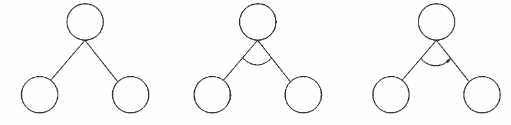
\includegraphics[scale=0.6]{resources/img/i8.png}
    \caption{攻击树基本结构}
  \end{figure}

\subsection{CVSS模型}

通用漏洞评分系统(CVSS)(2007 年完成,第 2 版)被认为是衡量软件漏洞相对严重性的规范,可应用于大
量系统,包括那些属于美国联邦机构的系统\cite{mell2007common}。
CVSS 由三个不同的度量组组成:基础、时间和环境。每一个都由它们自己的一套度量标
准组成。基本度量组可用于大多数情况,但也可以将其他值分配给其他度量组,以便为特定漏洞提供额
外的上下文。这些度量组可以描述如下:
\begin{itemize}
    \item  基础表示漏洞的特征,这些特征会随着时间和用户环境的变化而不断变化
    \item  时态表示漏洞随时间变化的特征,但不提及用户环境
    \item  环境表示与用户的特定环境相关和/或独特的漏洞特征
\end{itemize}

一旦为这些基本指标中的每一个分配了一个值,基本公式就会计算出一个范围从 0 到 10 的分数。根据所
有因素,从等式中创建一个向量,并将该向量输出为包含分配给每个指标的值的文本字符串,以便准确
传达如何为每个发现的漏洞得出分数。该过程如图 3.6 所示。
\begin{figure}
    \centering
    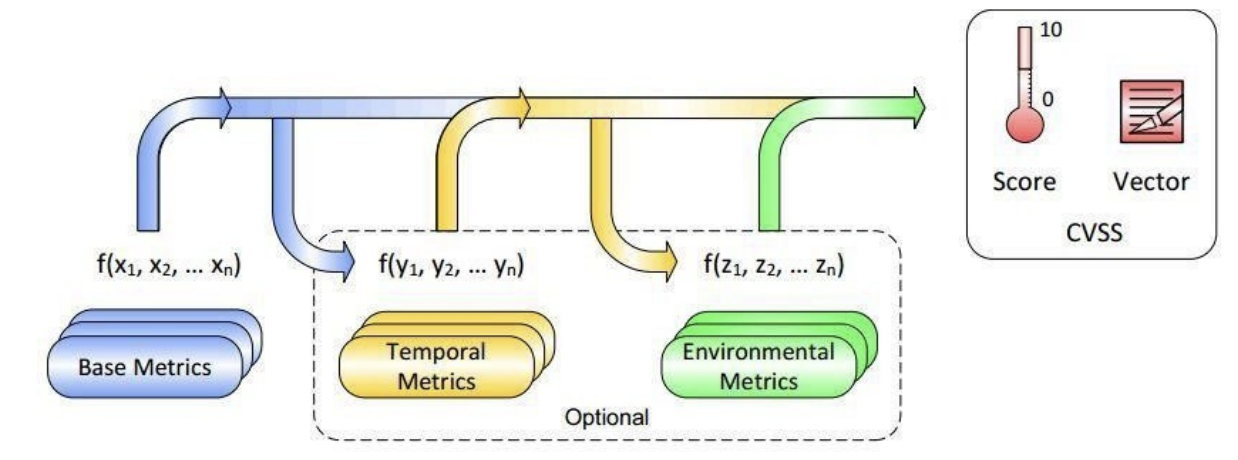
\includegraphics[scale=0.6]{resources/img/i9.png}
    \caption{CVSS的度量和方程组合起来创建矢量}
  \end{figure}

  \subsection{HEAVENS安全模型}
  如图3.7所示,HEAVENS安全模型旨在识别所有者、资产、风险、漏洞、对策、威胁代理和威胁,并将所有方面
整合在一起,以建立汽车行业的安全模型。此外,我们的目标是在汽车电子/电子系统的背景下研究来
自其他领域(例如,IT 安全、电信和国防)的安全模型。因此,在HEAVENS安全模型中,第一步是从涉众(即
所有者)的角度识别用例。用例随后被用于识别资产和威
胁,包括可能受到特定威胁影响的安全属性。在风险评估期间,威胁代理(攻击者)的角色以及攻击对特
定资产的影响已被考虑,以对威胁进行评级,即识别风险。这有助于确定安全要求和可能的对策,以解
决特定资产的特定威胁。

\begin{figure}
    \centering
    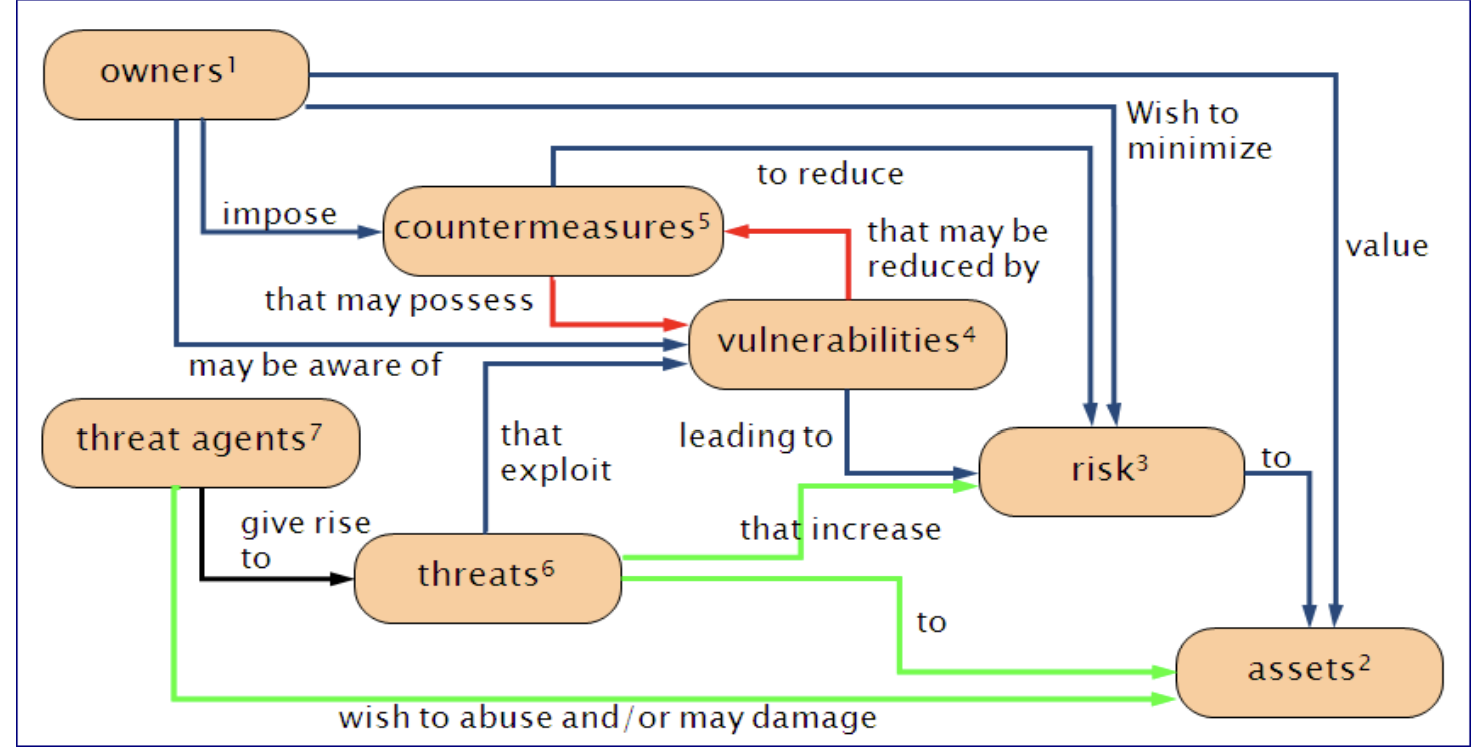
\includegraphics[scale=0.6]{resources/img/i10.png}
    \caption{典型的威胁风险评估图}
  \end{figure}

  HEAVENS安全模式的优势如下:

  \begin{itemize}
    \item  所提出的模型同样适用于各种道路车辆,例如客车和商用车。该模型考虑了广泛的利益相关方 (例
    如,原始设备制造商、车队所有者、车主、驾驶员、乘客等)。
    \item  时通过在汽车电子电气系统环境中应用微软的 STRIDE 方法实现的以威胁为中心的模型。它通过仅使用
    少数通用威胁类别,而不是考虑与资产相关的几乎无限的攻击可能性和攻击技术,来支持更好地理
    解可能的攻击的影响。
    \item  该模型在威胁分析期间建立了安全属性和威胁之间的直接映射。这有助于对特定资产的特定威胁的
    技术影响(机密性、完整性、可用性)进行可视化和早期评估。
    \item 该模型将安全目标(安全、财务、运营、隐私和法规)与风险评估期间的影响级别估计对应起来。这
    有助于了解特定威胁对相关利益方(例如 OEM)的潜在业务影响。
    \item 该模型符合成熟的行业标准和计划。例如,通用标准ISO-26262。这有助于
    重用其他研究领域已经存在的过程,例如,功能安全。它还提供了一个了解跨安全和安保领域的网
    络安全问题的机会。
\end{itemize}

HEAVENS安全模型的主要目标是推导出TOE的安全要求,即TOE的资产,类似于ISO-26262中所述的功能安全要求的概念。
为了实现这一点,我们为与构成 TOE 的资产相关的每个已识别的
威胁建立了一个安全级别。因此,HEAVENS安全模型包括威胁分析和风险评估。因此,“HEAVENS安全模型”指
的是威胁分析和风险评估,以便通过应用HEAVENS方法和工具支持来推导特定 TOE 的安全要求。
图 3.8 显示了HEAVENS安全模型的工作流程。它由三部分组成——威胁分析、风险评估和安全要求。
HEAVENS安全模型的工作流程如下:
\begin{itemize}
    \item  威胁分析–功能用例的描述(图中的 In\_01)是威胁分析流程的输入。威胁分析产生两个输出:(a)用例环境中每个资产的威胁和资产之间的映射(图中的Out\_01),
    以及(b)威胁和安全属性之间的映射(图中的Out\_02),以确定哪些安全属性由于资产环境中的特定威胁而受到影响。
    \item  风险评估—一旦确定了相关资产的威胁,下一步就是对威胁进行分级。这是在风险评估期间完成的。威胁和资产之间的映射与威胁级别(TL)(图中的 In\_03)和影响级别(IL)
    (图中的 In\_04)参数一起用作输入。作为风险评估的最终结果,我们为与TOE/用例的每个资产相关联的每个威胁确定安全级别(图中的 Out\_03)。
    \item  安全要求–最后,我们考虑威胁和资产之间的映射(图中的 Out\_02 是威胁分析的结果)以及安全级别(图中的 Out\_03 是风险评估的结果)来制定资产和 TOE 的安全要求。
    安全需求是资产、威胁、安全级别和安全属性的函数。请注意,安全级别根据与特定资产相关联的特定威胁的安全目标来考虑潜在的业务影响。
    衍生的安全要求处于 ISO-26262 功能安全要求的水平,属于概念阶段。之后,在产品开发阶段,需要根据高级安全需求派生出软件安全需求和硬件安全需求。
  \end{itemize}


\begin{figure}
    \centering
    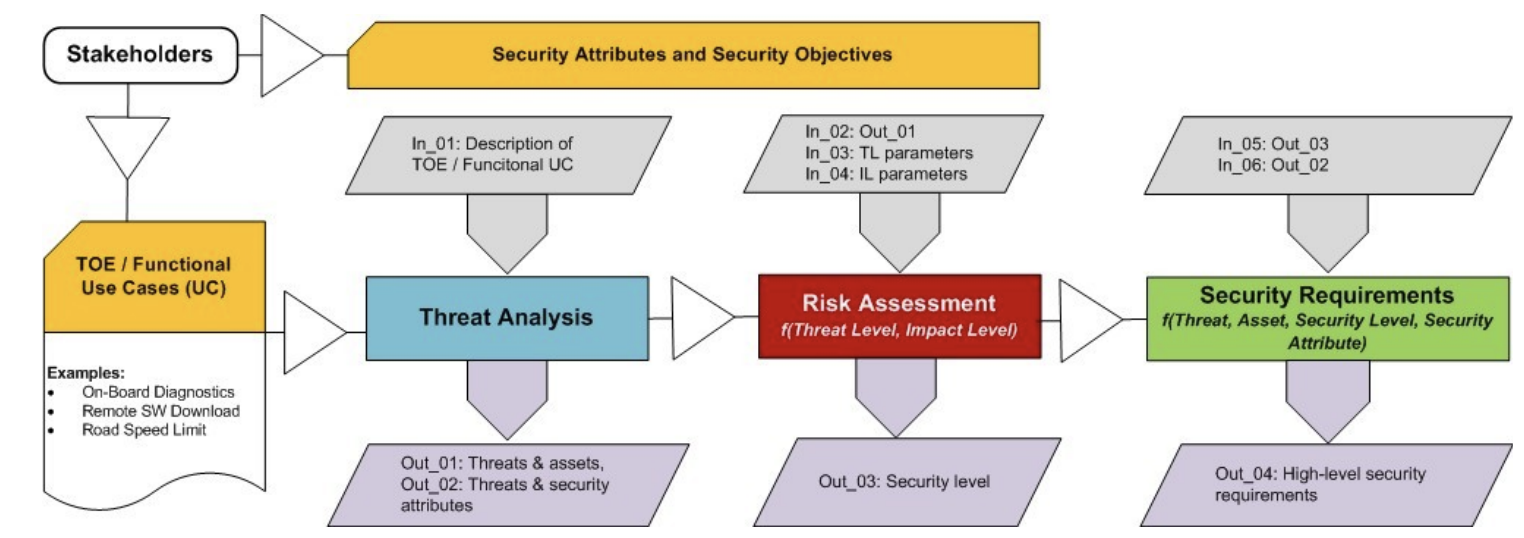
\includegraphics[scale=0.6]{resources/img/i11.png}
    \caption{HEAVENS安全模型工作流程图}
  \end{figure}

  \subsection{层次分析法和FAHP}
  这里我们介绍下层次分析法用于第四章进行新的安全模型的理论基础。
  AHP 是一种结合定性和定量分析的多目标决策分析方
法,由萨蒂在20世纪70年代提出\cite{saaty1990make}。这种方法的主
要思想是通过将复杂的问题分解成几个层次来比较每两
个决策元素的相对重要性,每个层次由有限数量的决策
元素组成。然后建立满足性质(2)(3)的判断矩阵。通过
计算判断矩阵的最大特征值和相应的特征向量,从两两
比较中间接评估不同元素的相对重要性。层次分析法的
特点是将人们的主观判断数学化,使决策更容易被接
受。AHP 的过程可分为以下步骤:
\begin{itemize}
  \item  构建一个问题的层次结构,包括一个目标、实现
  目标的要素以及对这些要素进行评分的评估标
  准。
  \item  将决策元素成对比较,根据标度准则确定相对
  重要性,然后构造一个判断。
  \item  计算每个元素的权重并检查判断矩阵的一致
  性。
  \item 通过比较综合重要性,根据所有备选方案的优先
  级做出最终决策。
\end{itemize}

然而,层次分析法难以检查判断矩阵的一致性,其一
致性判断准则缺乏科学依据。此外,当有许多评价指标
时,很难保证决策的一致性。在这种情况下,FAHP 应运而
生\cite{min1997fuzzy}。一种是基于模糊数的 FAHP,另一种是基于模糊判
断矩阵的。这里,我们使用后者。模糊判断矩阵应满足性
质(10)(11)。FAHP 的过程与层次分析法相同,但仍有两个
不同之处:
\begin{itemize}
  \item  建立的判断矩阵不同:层次分析法是判断矩阵,而
  FAHP 是模糊判断矩阵
  判断矩阵。
  \item  寻找矩阵中每个元素相对重要性的不同加权方
  法。
\end{itemize}


\subsection{本章小结}
本章首先介绍了智能网联汽车的主要攻击来源和攻击手段。然后介绍了三种类型的威胁方面。最后主要介绍智能网联汽车领域的威胁建模分析:
首先介绍传统的 STRIDE 模型,攻击树模型,CVSS 和 新型的HEAVES安全模型.此外还介绍了AHP和FAHP层次分析法用于定量分析。
详细阐述其建模原理和步骤,梳理威胁
的存在和建模流程,为第四章的全新SATT威胁建模方法提供理论基础,为第五章的实际商用攻击实例提供实例参考。